\section{Evaluation of main MPPT techniques\label{MPPTalgo}}

There are a variety of different techniques to find the maximum power point. Therefore only three different methods are used in this thesis, otherwise it would go beyond the scope of this work. These three methods are the perturb and observe constant voltage and incremental conductance. They were chosen because the perturb and observe and incremental conductance are the most used algorithms in commercial pv-panels. Constant voltage was selected as a comparison to methods that are not used so often. 

\subsection{Constant voltage algorithm}
Empirical experiments have shown that the voltage of the MPP has a linear dependence on the open circuit voltage at different ambient conditions. 
%%Equation Vmpp = k * V_oc
K represents a constant that depends on the characteristics of the respective pv panel. To determine the value for k, the voltage for mpp and idle must be recorded for each temperature and solar irradiation. According to different papers, this value lies between 70 and 80. The algorithm starts with the detection of the open circuit voltage and a predetermined k-value. In each iteration step the Vmpp with the equation is calculated first. Then the operating voltage is compared with the calculated voltage of the MPP. If the voltage is not equal, the constant k is changed for the next iteration step to reach the MPP. When the algorithm has reached the MPP, the algorithm is stopped, as you can see in the flowchart in the picture.
%%\cite{}

\begin{figure}[htbp]
	\begin{center}
		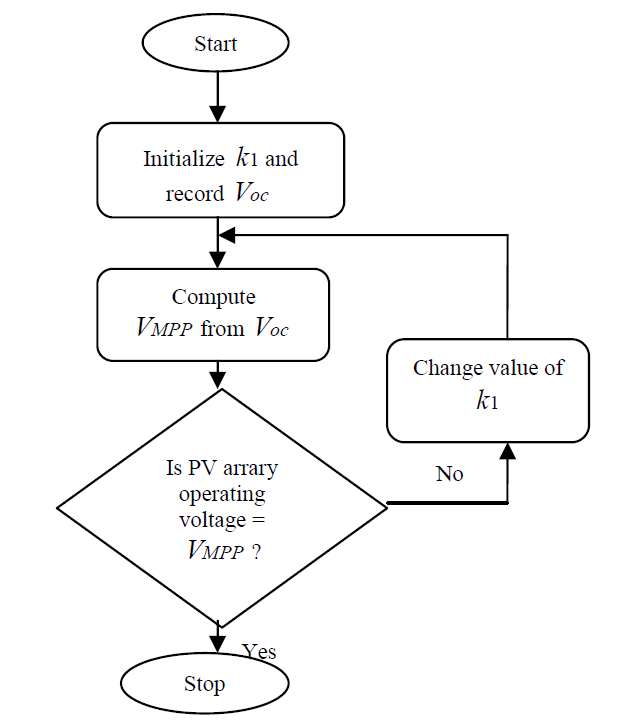
\includegraphics[width=0.7\textwidth]{../Pictures/P1/Flow_chart/Flow_chart_constant_voltage}
		\caption{flow chart from perturb and observe.picture should change }
		\label{fcconstantvoltage}
	\end{center}	
\end{figure}

\subsection{Perturb and Observe}
With perturb and observe, the currently measured power is periodically compared with the previous power. If the measured power is greater than the power from the previous measurement, the voltage is further increased to reach the MPP. If a power reduction is detected after the comparison, the voltage is reduced. The flowchart in the figure illustrates this method. The classical algorithm uses a fixed step to change the voltage. When the MPP is reached, otherwise the algorithm oscillates around the MPP.

\begin{figure}[htbp]
	\begin{center}
		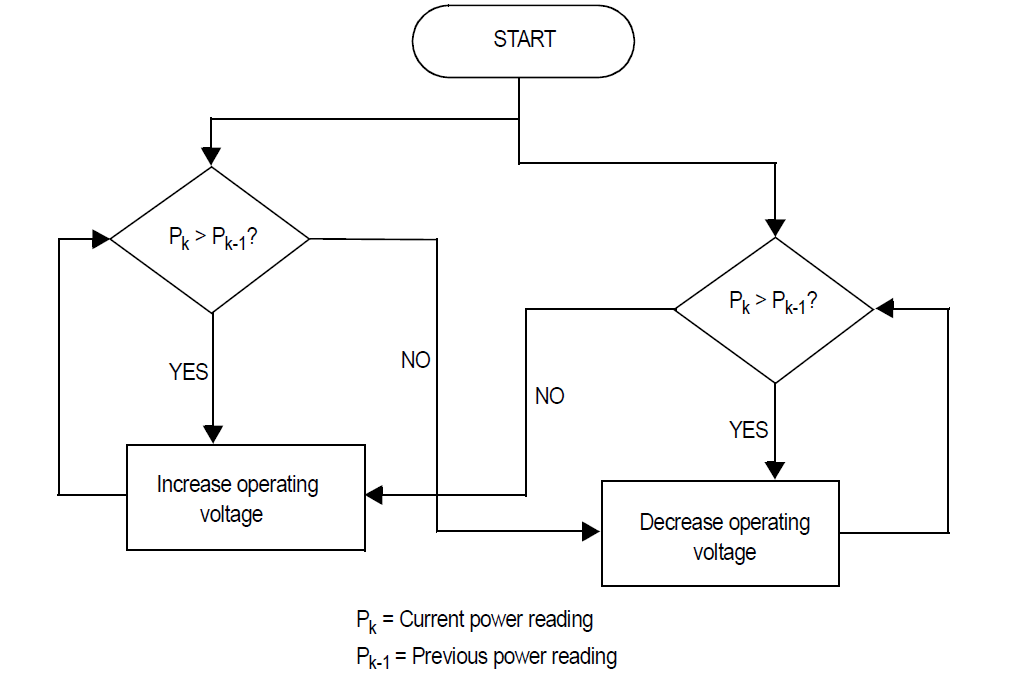
\includegraphics[width=0.7\textwidth]{../Pictures/P1/Flow_chart/flow_chart_perturb_observe}
		\caption{flow chart from perturb and observe.picture should change }
		\label{fcperturbandobserve}
	\end{center}	
\end{figure}

\subsection{Incremental conductancee}
The approach of incremental conductance is that the MPP is at the position where the derivative of the power after the voltage is 0. The left side of the MPP is the derivative greater than 0 and the right side is the derivative less than 0, which is described by the following equations. The algorithm compares the incremental conductance with the previous one to then increase (left side of MPP) or decrease (right side of MPP) the voltage.  After the MPP has been reached, the algorithm is stopped. There will be no oscillation around the MPP. If a change in the current is detected, the algorithm starts to find the MPP again, as you can see in the flowchart in the picture.

\begin{figure}[htbp]
	\begin{center}
		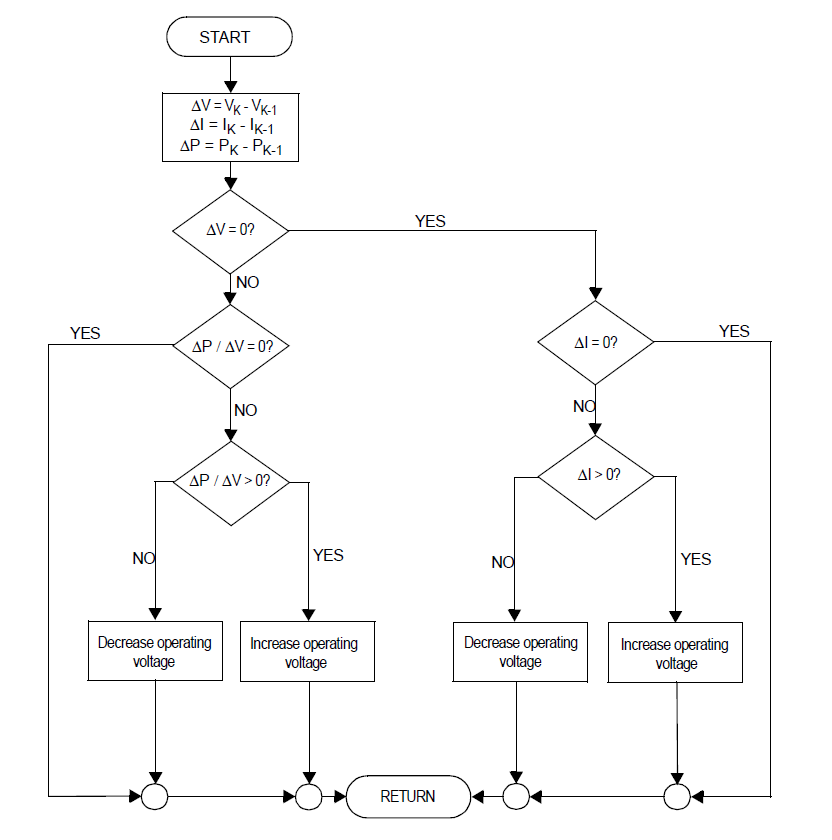
\includegraphics[width=0.7\textwidth]{../Pictures/P1/Flow_chart/flow_chart_incremental_conductance}
		\caption{flow chart from perturb and observe.picture should change }
		\label{fcinccon}
	\end{center}	
\end{figure}